\chapter{Result}
The focus of this thesis has been to minimize the amount of hardware 
usage, while trying to meet the timing constraints provided 
from the rest of the circuit. The clock frequency used on the FPGA has 
been 100 MHz. A throughput in the scale of Gbits/s is sufficient for the
current design.

The implemented scrambler processes 16 bytes of data in 11 clock pulses 
with a clock frequency of 94MHz, which would correspond 
roughly to a throughput of 1.16 Gbits/s. The reason why the design does 
not meet the frequency of the rest of the circuit is due to the 
critical path being too long. This is further discussed in section 
\ref{sec:c_path}.
The scrambler needs to process the key first, before being able to 
scramble data. A keyexpansion takes roughly 45 clock pulses, and is 
only performed when a new key is sent, which is very seldom. The 
scrambler then deals with 16 bytes of data on 13 clock pulses, but 
outputs 1 byte of data per clock cycle. This is done so that one byte 
of data from the scrambled package is read into a register on every 
clock pulse. When four bytes are collected the 32-bit output is sent 
out. 32-bits are processed at a time, since the data-bus is a 32-bit 
bus.

\section{Problems}
The main problems that were encoutered were:

\begin{itemize}
\item Not possible to get the license for CSA3
\item Small interrest for CSA3
\item Next to no documentation of the CISSA algorithm
\item Hard finding reliable test vectors
\item Merging
\item Timing
%\item Latches
\end{itemize}

When the Thesis was first started, the idea was that the CSA3 algorithm 
was to be implemented. However, licensing problems, and the fact that 
AES-128 in CBC-mode seemed like a better idea, led to a rework of the 
project.

Most of these problems are self-explanatory. The one that 
will be discussed here is the merging problem. This problem occured 
due to the fact that this design was a bottoms-up design, instead of 
the more common top-down design. This project was done by implementing 
low level entities first, that were to be used in higher hierarchies. 
Doing this caused some problems when merging entities into higher level 
blocks, since some signals, needed to be produced. This was not a huge 
problem, and only occurred on a few instances, but were rather 
troublesome at those times.

The pro of this method of working has been that it produced results 
quickly. The con is that a large portion of the time has been 
spent on going back to entities that were already functional, and 
reworking them by adding signals, and finding the right timing 
conditions to make sure that they provided nescessary information for 
entities higher up in the hierarchy.

Since the plan was to optimize this implementation to just meet the 
demands on speed, while trying to minimize the amount of hardware 
needed, timing was introduced into a few circuits that could have 
otherwise been completely combinatorial. This has, as expected, 
introduced quite a bunch of timing-issues. All of them seem to be gone 
now, but without more exhaustive testing, it is quite hard to know.

%% When the circuit was first synthesized, towards the end of the 
%% implementation, it was noted that the circuit synthesized a large 
%% amount of latches. This made the circuit take up roughly 15\% of the 
%% FPGA, and use 11830 Flip-Flops (FFs). At this time, there were roughly 
%% 3000 latches. When all of them were removed, the entire circuit 
%% used up roughly 8\% of the FPGA, and used about 4500 FFs instead. They 
%% appeared in the design due to a

This is the entire hardware usage, including the interface towards the 
FPGA, which is one of the reasons why it might appear large, when 
compared to other implementations.

\section{Hardware}
The top entity can be viewed in Figure \ref{b:scr}, and the rest of the 
entities are placed near the explanation of the entities in the 
following sections.

\begin{figure}
  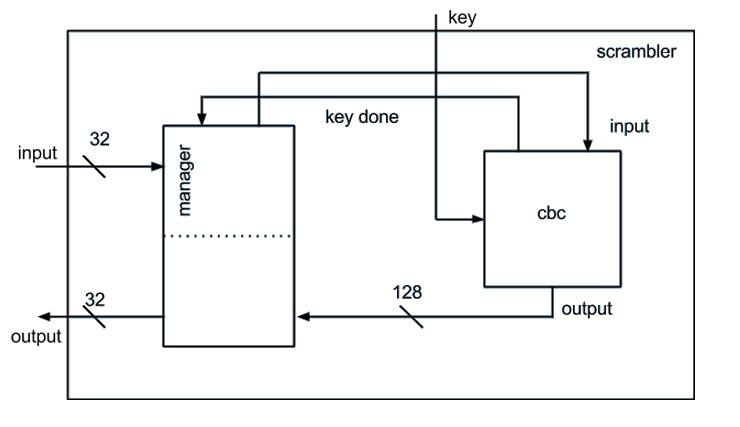
\includegraphics[width=\textwidth]{scrambler}
  \caption{The top entity}
  \label{b:scr}
\end{figure}

\subsection{Hardware usage}
The circuit that was first implemented has during the course of the 
project been optimized, after synthesis have been run, to either 
minimize hardware usage, or the speed of the circuit. A total of six 
synthesises were run. A table displaying the differences of the results 
can be viewed in figure \ref{table:synthesis}.
The optimizations performed between the synthesizes are discussed in 
this section.

\subsubsection{First synthesis}
This was the initial synthesis performed on the FPGA. This did not hold 
any interresting information, except indications about some minor 
errors that could be found in the initial version of the code.
%The circuit used up 15\% of the FPGA, and had quite a large amount of 
%unnescessary latches and FFs included. It used 11830 FFs, and roughly 
%3000 latches. The circuit was redesigned to remove the latches and ran 
%the second synthesis.

\subsubsection{Second synthesis}
%The circuit used up 8\% of the FPGA this time. 
What was noticed from the second synthesis was that the keyblock3 
entity, as well as keyblock1 entity seemed to use a lot of registers 
and multiplexers. It should be possible to replace them with RAMs or 
LUTs.

The maximum frequency obtained was 92MHz after this synthesis, where a 
lot of the minimum period was due to the routing of the circuit, which 
made up for 75\% of the period.

%% To be able to compare the third synthesis with this one, you need to 
%% know that the keyexpansion entity used 1538 D-type FFs and 16 
%% Comparators. It used up 176 8-bit registers, which were used by the 
%% expanded key.
Before running the next synthesis, it was noticed that the circuit 
waited for the expanded key to become completely filled before updating 
the output at one point. The expanded key was stored in a vector 
located in keyblock3 while it was updated. However, the expanded key 
used by other entities was not updated until the entire expanded key 
was filled, in keyblock3. Rewriting the code decreased the amount of 
registers by 176 8-bit registers, which could be removed by adding an 
enable signal. The enable signal tells the other entities when the 
expanded key is usable.

%% The entire circuit still used up roughly 8\% of the FPGA. The 
%% keyexpansion entity used 130 D-type FFs and 16 Comparators this 
%% time.
\subsubsection{Third synthesis}
The maximum frequency obtained this time was 94MHz. The number of 
Slice Registers went down from 4357 to 2945, and the percentage of 
Slice Registers decreased from 3\% usage to 2\% usage.

The keyblock3 module seems to be using the most hardware from what can 
be seen. It uses roughly 1302 multiplexers, which should be reducable.

\subsubsection{Fourth synthesis}
The next synthesis was made after the state2data module was rewritten, 
to remove yet another signal. This should have decreased the design by 
a 128-bit register. It was mostly done to try to allow for a synthesis 
of the module, while also reducing hardware usage. This would decrease 
the number of D-type FFs by yet another 128. A comparison between 
report 3 and 4 displays a decrease from 130 D-type FFs to 2 D-type FFs, 
which confirms that 128 FFs were removed.

The maximum frequency obtained this time was 94MHz. The number of 
FFs went from 2945 to 2817. However, this did not affect the number of 
Slice Registers.

%The circuit still uses roughly 8\% of the hardware on the FPGA.

\subsubsection{Fifth synthesis}
During the fifth synthesis, it was noted that two reports were made 
during synthesis and optimization. Those were a Synthesis Report as 
well as a Place and Route Report. The ones that have been examined 
this far have been the Synthesis Reports, and to make sure that 
there are not any huge gaps in numbers between the reports, they will 
be the ones analyzed, and not the Place and Route Reports. Many of the 
entities can not be mapped seperately, due to the amount of IOs on the 
FPGA, compared to the number of IOs required by the modules.

The third synthesis was performed on each block seperately, to find out
where optimization might be performed. The usage can be viewed in Table 
\ref{synt:fifth}.

%
\newcommand{\MyIndent}{\hspace*{0.2cm}}%

\begin{longtable}{ l | c | c }
  Entity & Slice LUTs out of 63288 & Slice Registers out of 
  126576 \\ \hline
  scrambler              & 5167 & 2817 \\
  \MyIndent \triangleright manager      &  858 &  699 \\ 
  \MyIndent \triangleright cbc          & 4321 & 2127 \\

  \MyIndent \MyIndent \triangleright cipher       & 4229 & 1994 \\

  \MyIndent \MyIndent \MyIndent \triangleright keyexpansion & 2914 
  & 1601 \\

  \MyIndent \MyIndent \MyIndent \MyIndent \triangleright keyblock1 
  & 689 & 0 \\
  \MyIndent \MyIndent \MyIndent \MyIndent \triangleright keyblock2 
  & 208 & 9 \\

  \MyIndent \MyIndent \MyIndent \MyIndent \MyIndent \triangleright 
  demux & 32   & 0 \\
  \MyIndent \MyIndent \MyIndent \MyIndent \MyIndent \triangleright 
  keycore & 183 & 9 \\

  \MyIndent \MyIndent \MyIndent \MyIndent \MyIndent \MyIndent 
  \triangleright ctr & 14 & 9 \\
  \MyIndent \MyIndent \MyIndent \MyIndent \MyIndent \MyIndent 
  \triangleright rotw & 0 & 0 \\
  \MyIndent \MyIndent \MyIndent \MyIndent \MyIndent \MyIndent 
  \triangleright sbox & 128 & 0 \\
  \MyIndent \MyIndent \MyIndent \MyIndent \MyIndent \MyIndent 
  \triangleright rcon & 40 & 0 \\

  \MyIndent \MyIndent \MyIndent \MyIndent \triangleright keyblock3 
  & 1854 & 1365 \\

  \MyIndent \MyIndent \MyIndent \triangleright data2state & 0 
  & 0 \\
  \MyIndent \MyIndent \MyIndent \triangleright round & 1535 & 272 \\

  \MyIndent \MyIndent \MyIndent \MyIndent \triangleright subbytes 
  & 512 & 0 \\
  \MyIndent \MyIndent \MyIndent \MyIndent \triangleright shiftrows 
  & 0 & 0 \\
  \MyIndent \MyIndent \MyIndent \MyIndent \triangleright mixcolumns 
  & 176 & 0 \\
  \MyIndent \MyIndent \MyIndent \MyIndent \triangleright addkey & 128 
  & 0 \\

  \MyIndent \MyIndent \MyIndent \triangleright state2data & 1 & 2 \\

  \caption{Hardware usage of entities}
  \label{synt:fifth}
\end{longtable}

The plan was to try to reduce the critical path by inserting FFs in the 
middle of it and then run another synthesis. This would have increased 
the hardware by a lot of FFs, but also increased the maximum frequency. 
This was hard to do due to timing issues in the key generation. Adding 
some signal delay after keyblock3 would have reduced the critical path, 
but also changed a lot of timing constraints in the keygeneration 
block FSM. Therefore a decision was made to change the \emph{User 
Constraints File} (UCF) instead of spending the time trying to 
decrease the critical path, only to increase the amount of hardware.

Running the synthesis with an UCF is supposed to make the synthesis 
program optimize the layout of the circuit according to a number of 
constraints provided by the user. The constraint made here, was to 
reach the desired frequency of 100 MHz. However, no information about 
whether that frequency could be reached or not was found in the reports.

\subsubsection{Sixth synthesis}
The final place and route yielded the following results:
\begin{verbatim}
Number of Slice Registers: 2,805 out of 126,576    2%
Number of Slice LUTs:      4,930 out of  63,288    7%
\end{verbatim}

There is a difference of one register between the fifth and sixth 
synthesis reports. That register is most likely a residue after the 
attempts to reduce the critical path, and can be disregarded.

\subsubsection{Comparison of synthesis results}
The most interresting numbers from the synthesizes are the number of 
LUTs used, number of ROMs and number of FFs. However, only one ROM has 
been implemented in this design, which was present in all synthesizes, 
which is why it will not be included in the comparison.
\begin{figure}[h!]
  \begin{equation}
    \begin{array}{l | l | l | l | l | l}
      & Second & Third & Fourth & Fifth & Final \\ \hline
      LUTs       & 5121   & 5167  & 5167   & 5167  & 5167  \\ \hline
      Registers  & 4537   & 2945  & 2817   & 2817  & 2818  \\
    \end{array}
  \end{equation}
  \caption{Synthesis results}
  \label{table:synthesis}
\end{figure}

%Noteworthy is that the number of LUTs increases between the second and third synthesis, and does not decrease thereafter. The reason why this 
%happens is possibly due to routing of signals, and 
\Warning[Todo]{Why is this?}

\section{Further development}
There are, as usual, an amount of optimization that could be performed 
on the circuit. They consist of optimization of code, as well as some 
deeper research into how to rewrite VHDL code to turn the registers in 
this implementation into RAMs, ROMs or LUTs.

\subsection{Rijndael's S-Box}
The Rijndael Sbox implemented in this design does not synthesize into a 
ROM, which it should be able to do. Other than a ROM, it should also be 
able to be synthesized into a couple of LUT6.
It has not been possible to find out why the code was implemented into 
registers instead of more efficient solutions.

\subsection{Critical Path}\label{sec:c_path}
To increase the maximum frequency of the circuit, the critical path 
needs to be decreased. This is done by adding FFs in the middle of the 
critical path. This will be hard to solve, due to the complexity of the 
keyexpansion, and would increase the amount of hardware as well as the 
complexity of the circuit if FFs were to be added.

The decision whether to reduce the critical path, or not, is a hard 
decision due to the amount of hardware that might need to be added to
increase the frequency. However, since LUTs and FFs are located on 
same slice, it is not sure wether the design would use more slices or 
not.

%% \subsection{HARDUNÅGOTMERDUVILLFÖRBÄTTRA?}

\section{Implementation}
This design is very hierarchical. The top layer is an aes128 block in 
CBC-mode. It takes an input TS-packet, selects data from it which it 
scrambles, and then outputs the data in the form of a TS-packet once 
again.

The scrambler (Figure \ref{block:scrambler}) consists of two entities. 
An entity which is called the cbc-entity, which deals with the 
scrambling of the received data. The other entity is a data-manager. 
The manager deals with reading data from the interface towards the rest 
of the FPGA as well as sending the right data-bits to the CBC-entity. 
It also tells the CBC-entity how to handle the data, since different 
things are to be done depending on if the data is the first data packet 
sent, or not.

\begin{figure}[h!]
  \centering
  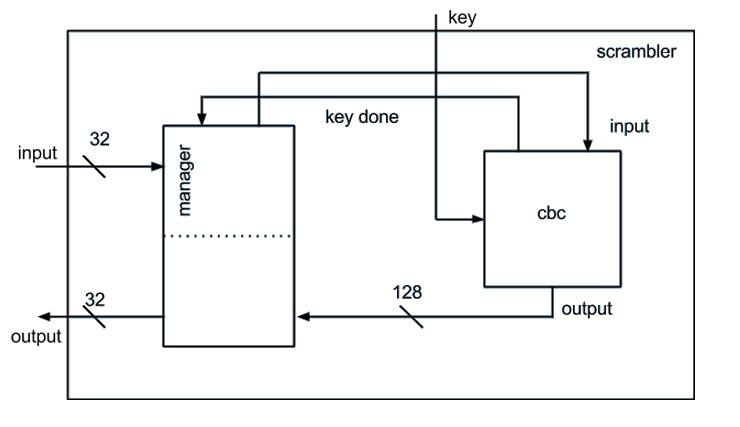
\includegraphics[width=0.75\textwidth]{scrambler}
  \caption{Scrambler-block}
  \label{block:scrambler}
\end{figure}

\subsection{Manager entity}
The manager (Figure \ref{block:manager}) consists of a FIFO, an FSM and 
a couple of registers. The FIFO is needed since the data sent to the 
scrambler from the FPGA is sent in bursts. The FIFO therefore writes 
the data bursts into a memory, from which it later reads, processes and 
sends the data to the CBC-entity. The data written to the FIFO is 
written in packets of 32 bits, but are read 8 bits at the time. The 
manager looks through the data packets to see if there is an adaptation 
field or not, since that changes the way that data is handled. The 
payload is written to the first set of registers as the data is found, 
and then sent to the next set of registers. This is simply done to 
allow the manager to deal with two sets of data in parallell. When the 
packet is ready to be sent, a flag is set and the data is sent to the 
CBC-entity. 

\begin{figure}[h!]
  \centering
  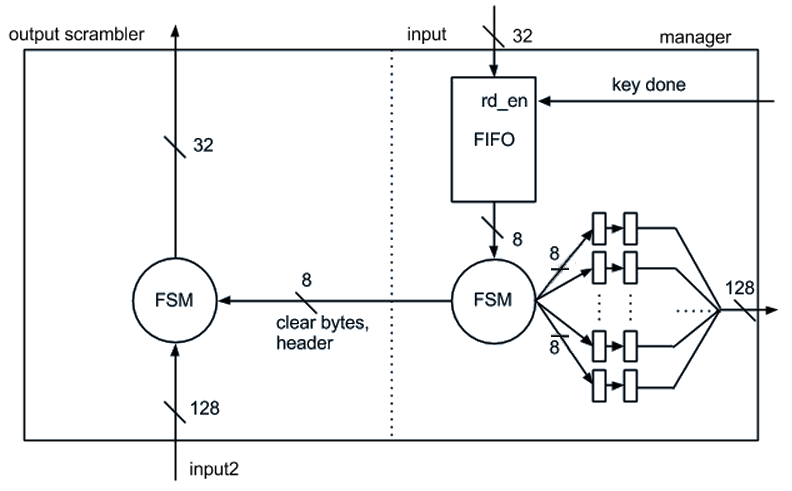
\includegraphics[width=0.75\textwidth]{manager}
  \caption{Manager-block}
  \label{block:manager}
\end{figure}

\subsection{CBC entity}
The CBC-entity (Figure \ref{block:cbc}) consists of three small 
entities. An XOR, a multiplexer and a cipher-entity. The multiplexer is 
needed since the first plaintext should be sent to the XOR together 
with an IV. For the rest of the plaintexts contained within the same 
TS packet, the output ciphertext should be used instead of the IV. 
There is only going to be one aes128 cipher in the CBC-entity, in order 
to save hardware. It will be run in sequence instead of in parallell, 
even though it might reduce the maximal speed of the circuit.

\begin{figure}[h!]
  \centering
  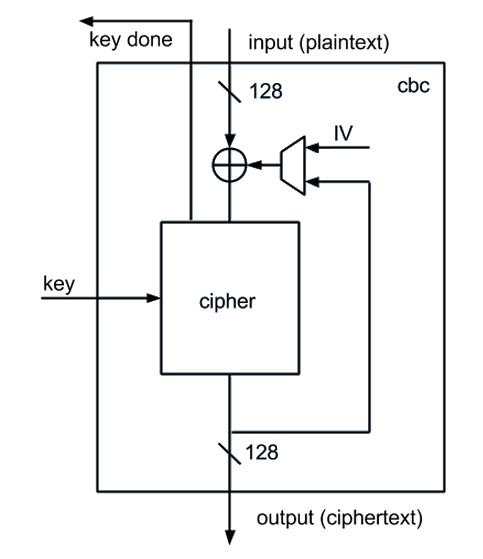
\includegraphics[width=0.75\textwidth]{cbc}
  \caption{CBC-block}
  \label{block:cbc}
\end{figure}

\subsection{Cipher entity}
The aes-128 cipher-entity (Figure \ref{block:cipher}) consists of 4 
components. The data2state entity, which transforms the array into a 
matrix of data. A keyexpansion entity, which takes an input of a key, 
and generates an extended key as an output. An entity, which was named  
rounds, that deals with the encryption of the 16 byte data blocks. 
And finally a state2data entity, which transforms the data-matrix into 
an array once again. The cipher entity itself keeps track of timing 
mainly between the keyexpansion and the round entity. It uses itself of 
an FSM to make sure that the round entity is provided with the correct 
roundkey at the right time, and data is output when it is scrambled. 
What can not be seen in figure \ref{block:cipher} is that the 
keyexpansion entity also sends an enable signal, that tells the cipher 
entity that the expanded key is complete.

\begin{figure}[h!]
  \centering
  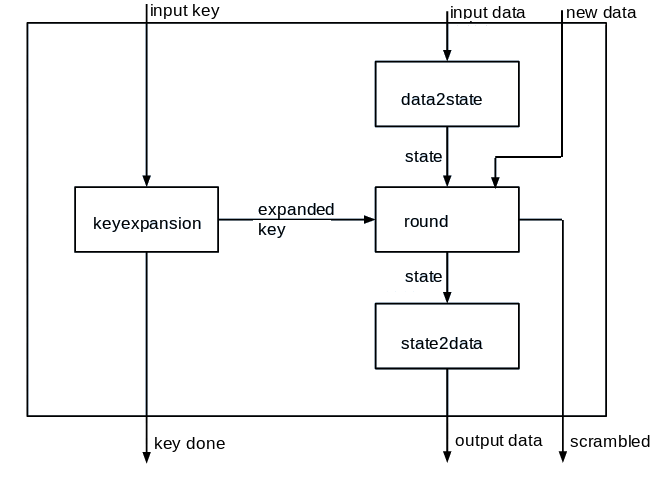
\includegraphics[width=0.75\textwidth]{cipherblock}
  \caption{Cipher-block}
  \label{block:cipher}
\end{figure}

\subsection{Keyexpansion entity}
The keyexpansion-entity (Figure \ref{block:keyexpansion}) is divided 
into 3 keyblock entities. The first keyblock entity decides what 4 
bytes of the expanded key are to be expanded. The second keyblock 
entity (Figure \ref{block:keyblock2}) contains the keycore, which is 
only performed on every 4th set of 4 bytes, and a demux entity. 
The third keyblock entity performs an xor between either the first or 
second keyblock depending on if the keycore was supposed to be run. It 
also increments the internal counter, which is used as an index when 
accessing and generating the 4 byte blocks of data.

The FSM seen in figure \ref{block:keyexpansion} keeps track of when the 
key generation is done, and and produces a lock signal at that time. 
The lock signal is used by keyblock3 to produce the done signal, that 
is passed to other entities. 
The FSM also keeps track of when a new key is received, and forces a 
reset of keyblock2 and keyblock3, since they are not entirely 
combinatorial. The reset\_i signal is the force reset signal. 

\begin{figure}[h!]
  \centering
  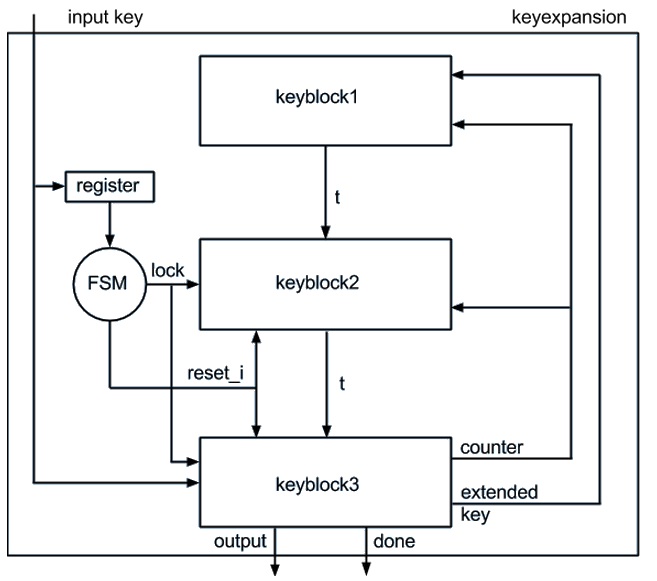
\includegraphics[width=0.75\textwidth]{keyexpansion2}
  \caption{Keyexpansion-block}
  \label{block:keyexpansion}
\end{figure}

\begin{figure}[h!]
  \centering
  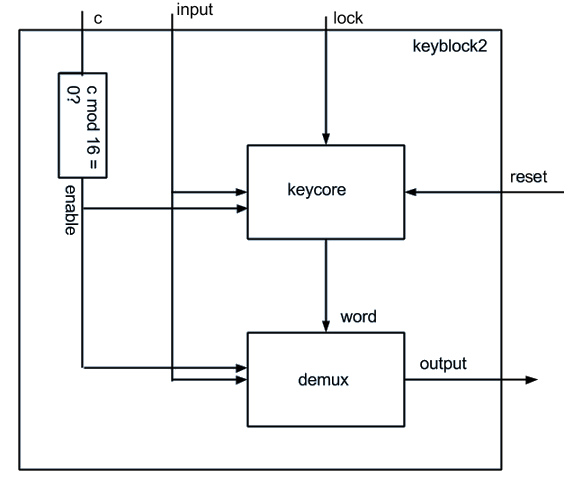
\includegraphics[width=0.75\textwidth]{keyblock2}
  \caption{Keyblock2-block}
  \label{block:keyblock2}
\end{figure}

\subsubsection{Keycore entity}
The keycore entity consists of four entities. Rotword, Sbox, Rcon and a 
counter. The counter is used to get the right data-byte from the Rcon 
entity, and the index is only used in the keycore, and is thus best 
suited to be placed inside the keycore entity. Rotword rotates the 
bytes of the input one step to the left through a simple left shift. 
Sbox replaces the input bytes according to the Rijndael Sbox, through 
a LUT. The Rcon entity both collects the correct rcon value from a 
precalculated vector, as well as inputs it into an xor together with 
the input.

\subsection{Round entity}
The round-entity (Figure \ref{block:round}) consists of four entities. 
Subbytes, shiftrows, mixcolumns and addroundkey. Addroundkey is a 
somewhat special XOR. Subbytes is an Rijndael Sbox, which takes an 
input 16-byte state, substitutes it, and outputs another 16-byte state. 
Shiftrows transposes the rows of the second, third and fourth row of 
the state. Last, but not least, is the mixcolumns entity. It consists 
of 16 mulblock entities. The input state of mixcolumns is split into 
columns, and each column is sent to a mulblock entity, which multiplies 
the inputs with 1, 2 or 3, then performs a bitwise XOR on them, 
outputting the result of the XOR. The function of the mixcolumns block 
is a rather complex matrix multiplication.

\begin{figure}[h!]
  \centering
  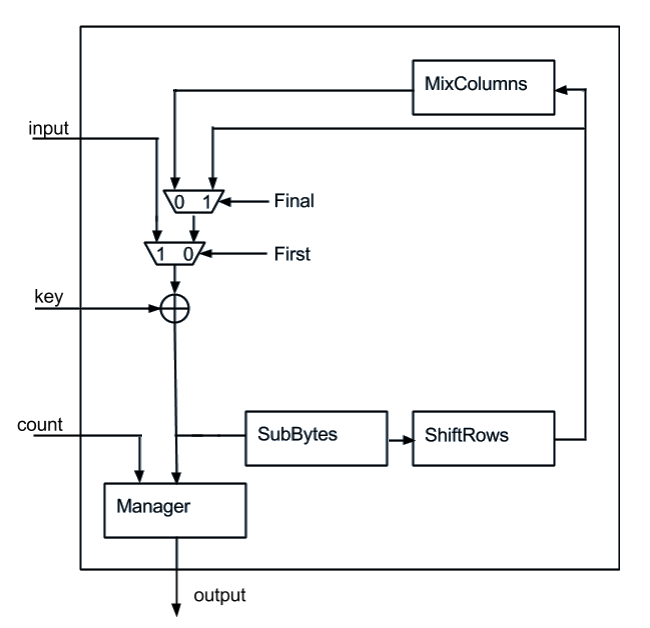
\includegraphics[width=0.75\textwidth]{round}
  \caption{Round-block}
  \label{block:round}
\end{figure}

\subsubsection{Addroundkey entity}
Addroundkey is an entity which takes different inputs depending on 
what round is currently being dealt with. On the first round, 
addroundkey takes the input to the round entity. On the last round, it 
takes the output from the subbytes entity. The input to addroundkey is 
the output from mixcolumns the rest of the time.

\subsubsection{The mulblock entity}
The mulblock entity consists of one mul3 entity and one mul2 entity, 
which performs a special kind of hardware multiplication of 3, and 2, 
on the input. It also takes two inputs which it leaves alone. The four 
results are then XOR:ed with eachother, and returned to the mixcolumns 
entity. The result is then input into the correct index in the matrix. 

Mul3 means multiplication with 3, and mul2 means multiplication with 2. 
A multiplication with 2 is a left-shift, followed by an XOR with the 
fix value 0x1B if the shifted value exceeds 0xFF. A multiplication with 
3 is the same as a multiplication with 2, followed by an XOR with the 
input value.

\section{Tests}
All of the entities in the design have been simulated and evaluated 
seperately before being merged and tested together, to make sure that 
they had the desired functionality both seperately and when combined 
together. The simulations for the seperate blocks are trivial, and 
therefore not included in the report.

Figure \ref{test:1} through \ref{test:3} are tests performed on the 
complete aes-128 block, before CBC-mode. In the figures, in\_key is the 
input key to be extended and used, and datapacket is one packet from a 
TS. Test vector 1 and 2 are taken from \citep{AES:2001}, while test 
vector 3 is generated using a webpage.

\emph{Test vector 1 (Figure \ref{test:1})}\\
Input key: 2b 7e 15 16 28 ae d2 a6 ab f7 15 88 09 cf 4f 3c\\
Plaintext: 32 43 f6 a8 88 5a 30 8d 31 31 98 a2 e0 37 07 34\\
Ciphertext: 39 25 84 1d 02 dc 09 fb dc 11 85 97 19 6a 0b 32

\begin{figure}
  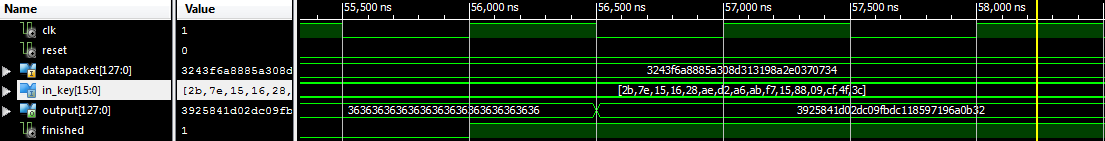
\includegraphics[width=\textwidth]{successtv1}
  \caption{Test vector 1}
  \label{test:1}
\end{figure}

\emph{Test vector 2 (Figure \ref{test:2})}\\
Input key: 00 01 02 03 04 05 06 07 08 09 0a 0b 0c 0d 0e 0f\\
Plaintext: 00 11 22 33 44 55 66 77 88 99 aa bb cc dd ee ff\\
Ciphertext: 69 c4 e0 d8 6a 7b 04 30 d8 cd b7 80 70 b4 c5 5a

\begin{figure}
  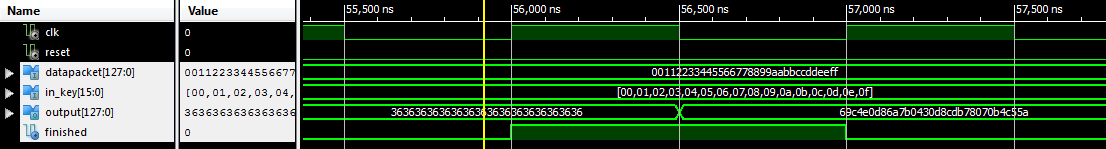
\includegraphics[width=\textwidth]{successtv2}
  \caption{Test vector 2}
  \label{test:2}
\end{figure}

\emph{Test vector 3 (Figure \ref{test:3})} \\
Input key: 10 20 30 40 50 60 70 80 90 a0 b0 c0 d0 e0 f0 bb\\
Plaintext: 00 11 22 33 44 55 66 77 88 99 aa bb cc dd ee ff\\
Ciphertext: bf 99 1f aa 8b 0f e6 48 36 46 a0 2d 33 9e de a5

\begin{figure}
  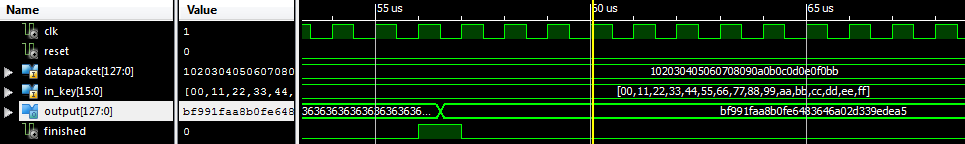
\includegraphics[width=\textwidth]{successtv3}
  \caption{Test vector 3}
  \label{test:3}
\end{figure}

\section{Comparison to other implementations}
Since there exists more implementations of the AES-128 algorithm, an 
analyzis between the implementations is interresting. To be noted is 
that this report and implementation have been made in effort to 
minimize the hardware usage, while achieving a suitable frequency.
Since it is possible to achieve an entirely combinatorial AES128 
scrambler, as well as pipelined version, the focus has been to try to 
find an implementation as similar as this one as possible, to compare 
results. 

Note that this implementation has got a couple of entities, that are 
usually not present in these kinds of designs, in order to allow 
insertion of the implementation into the FPGA used by WISI.

The design implemented in this thesis scrambles a block of 16 bytes 
of data in 13 clock pulses. It uses 4930 LUTs, occupies 1727 slices and 
can be run at a maximum frequency of 94 MHz. The circuit is implemented 
on a Xilinx Spartan-6.

This can be compared to the Fast AES XTS/CBC implementation (Helion) 
made by Xilinx themselves. It uses 1041 slices and 4047 LUTs with a 
maximum frequency of 130 MHz. \cite{Xilinx:AES} 

The implementation by Xilinx uses custom FPGA optimization techniques 
through hand crafted macros. A comparison between the two 
implementations can be found in table \ref{fig:imp_diff}. When these 
two implementations are compared, the most important difference is the 
frequency at which the two circuits can be run. The amount of LUTs that 
are used does in fact not tell a lot, since a LUT is said to be used
even if just a small part is used in the circuit. Also, LUTs can spand 
from anything between The same goes for slices. If only one LUT in a 
slice is used, it still counts the slice as used. 
%Considering the Xilinx version being implemented to optimize the LUT and slice usage, the data has to be seen critically.

The percentage row in table \ref{fig:imp_diff} indicates how many more 
percent LUTs and slices that are used in this implementation compared 
to the Xilinx implementation. However, the frequency shows how much 
higher the frequency of the Xilinx implementation is.

\begin{table}[h!]
  \centering
  \begin{array}{| l | l | l | l |}
    \hline
    & Slices & LUTs & Frequency (MHz) \\ \hline
    This & 1727 & 4930 & 94 \\ \hline
    Xilinx & 1041 & 4047 & 130 \\ \hline
    Percentage & 65\% & 21.8\% & 27.7\% \\ \hline
  \end{array}
  \caption{Comparison between implementations}
  \label{fig:imp_diff}
\end{table}

\section{Discussion}
The main reason for choosing a bottoms-up methodology, was since the 
functionality of the smaller blocks were very basic, but the timing was 
rather complex. In addition to the fact that there were no concrete 
guidlines, performing the work on the smaller entities, and then 
implementing the higher ones minimized the probability of performing 
tasks that were to be discarded in later stages of the implementation.

\section{Conclusions}
One of the first things noticed during this thesis was that industrial
secrecy can put a quick halt to projects. A license had to be written 
and approved by ETSI before WISI Norden was allowed information about 
the specifications of one of the algorithms that were supposed to be
analyzed. Due to restrictions, this could not be done, meaning that 
this specific analyzis came to a halt before it even started. This 
led to the comparison between a software- and hardware-friendly 
algorithm becoming impossible to do. 

While WISI Norden and ETSI were discussing the license, specifics about 
the CSA3 and CISSa algorithms were investigated, since those were the 
ones to be analyzed. From the little information available about 
the CSA3, only the names of the two ciphers were possible to find. 
Since one of the two ciphers in the CSA3 algorithm corresponded to one 
of the ciphers in the CISSA algorithm, this cipher was examined as much 
as possible. This was the AES-128 cipher.

Both the key generation, and the functionality of the entities in 
AES-128 algorithm could be found in litterature, since the AES 
encryption is a public algorithm. From what could be found out about 
the CISSA algorithm, through an official ETSI journal, it seemed to 
just use the AES-128 algorithm, but in a certain mode, with a specific 
Initialization Vector.
